%%\subsection{Results for $C_{DS}=0.0$}
%The following results are for a run with the following input conditions:
%\begin{longtable}[c]{A{3.0cm}  A{3.0cm}}
%    \caption{Input list for $C_{DS}=0$ test}    \\  \hline
%        \textbf{Parameter}      &       \textbf{Value}      \\  \hline
%    \endfirsthead
%    \caption{Input list for $C_{DS}=0$ test~(continued)}    \\  \hline
%        \textbf{Parameter}      &       \textbf{Value}      \\  \hline
%    \endhead
%        $N$                 &   64      \\
%        $t_{final}$         &   100.0   \\
%        $C_{DS}$            &   0.0     \\
%        $C_{BS}$            &   1.0     \\
%\end{longtable}
%
%%\newpage
%
%\begin{figure}[H]
%    \begin{subfigure}[H]{0.45\textwidth}
%        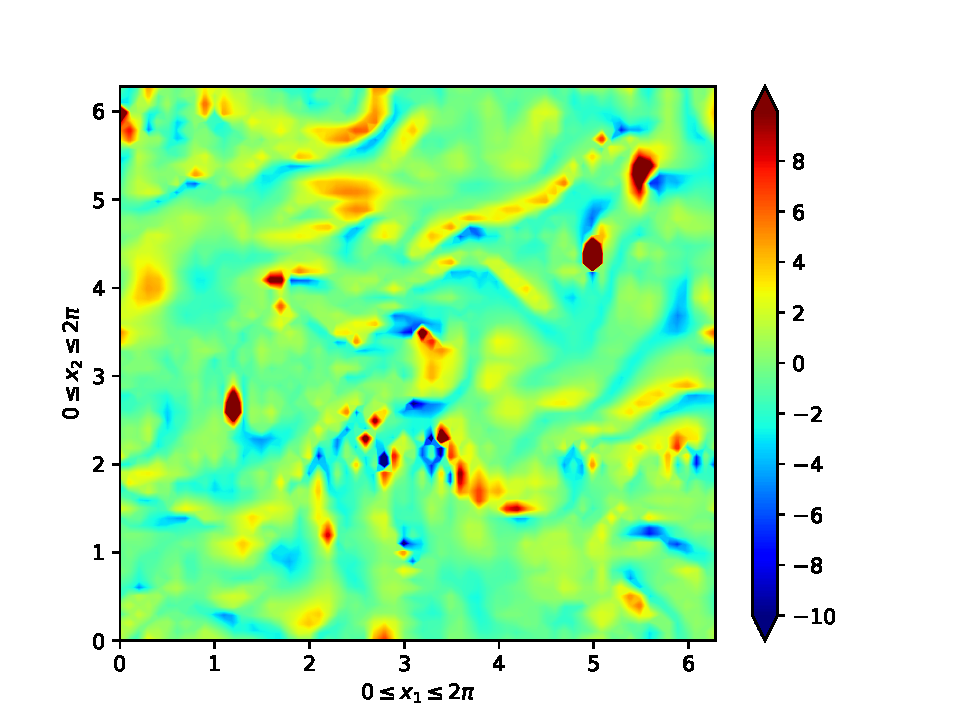
\includegraphics[height=1.75in]{media/run-cds-00/ke-RHS-CDS-00}
%        \caption{$\frac{1}{k} \frac{Dk}{Dt}$}
%    \end{subfigure}
%    ~
%    \begin{subfigure}[H]{0.45\textwidth}
%        \includegraphics[height=1.75in]{media/run-cds-00/enstrophy-RHS-CDS-00}
%        \caption{$\frac{1}{\Omega} \frac{D \Omega}{Dt}$}
%    \end{subfigure}
%    \newline
%    \begin{subfigure}{0.45\textwidth}
%        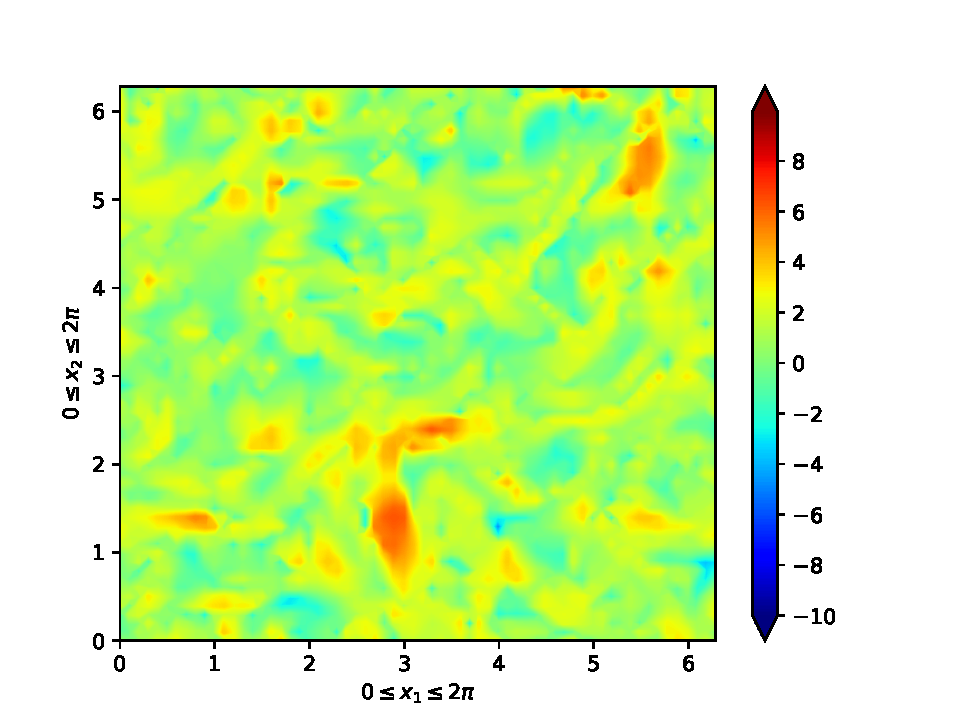
\includegraphics[height=1.75in]{media/run-cds-00/A-enst-CDS-00}
%        \caption{$A_{\Omega}$}
%    \end{subfigure}
%    ~
%    \begin{subfigure}{0.45\textwidth}
%        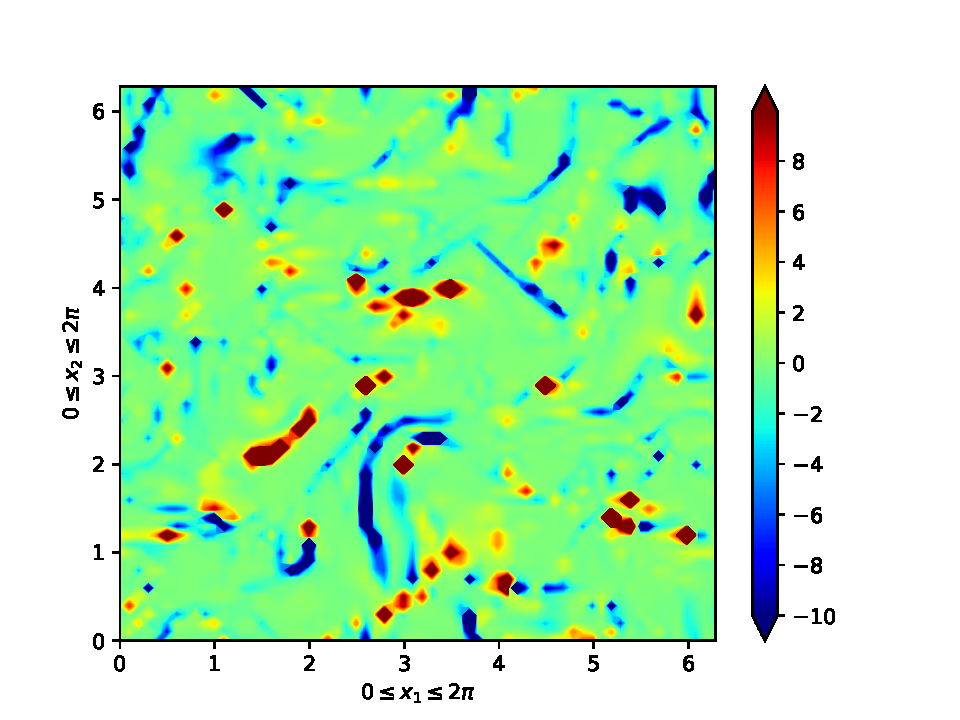
\includegraphics[height=1.75in]{media/run-cds-00/trans-enst-CDS-00}
%        \caption{$C_{\Omega}$}
%    \end{subfigure}
%    \newline
%    \begin{subfigure}{0.45\textwidth}
%        \includegraphics[height=1.75in]{media/run-cds-00/prod-enst-CDS-00}
%        \caption{$P_{\Omega}$}
%    \end{subfigure}
%    ~
%    \begin{subfigure}{0.45\textwidth}
%        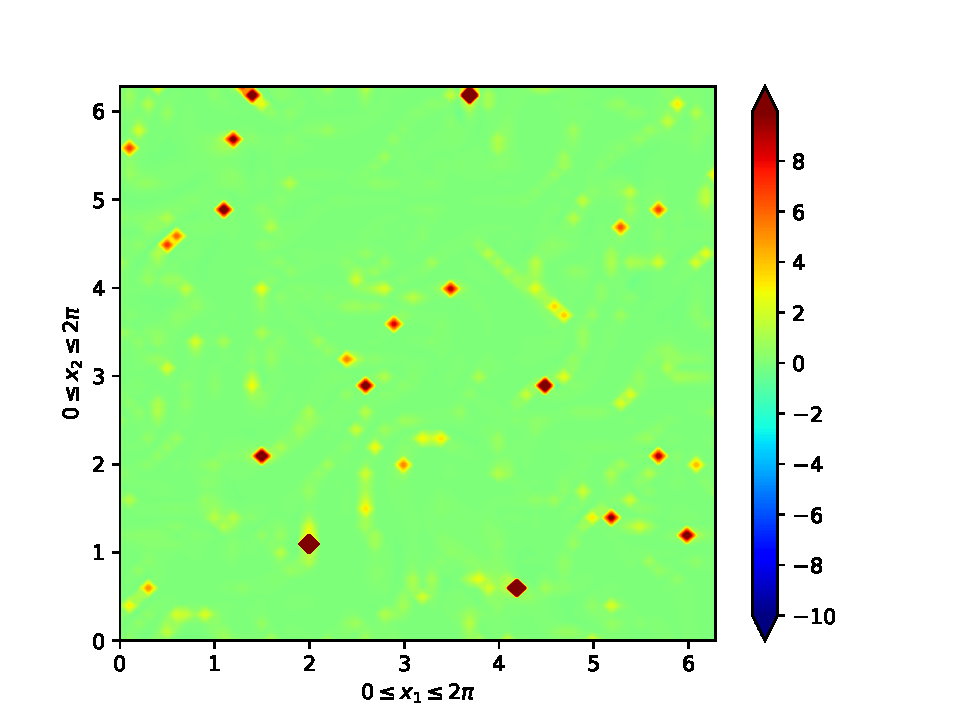
\includegraphics[height=1.75in]{media/run-cds-00/B-enst-CDS-00}
%        \caption{$B_{\Omega}$}
%    \end{subfigure}
%    \newline
%    \begin{subfigure}{0.45\textwidth}
%        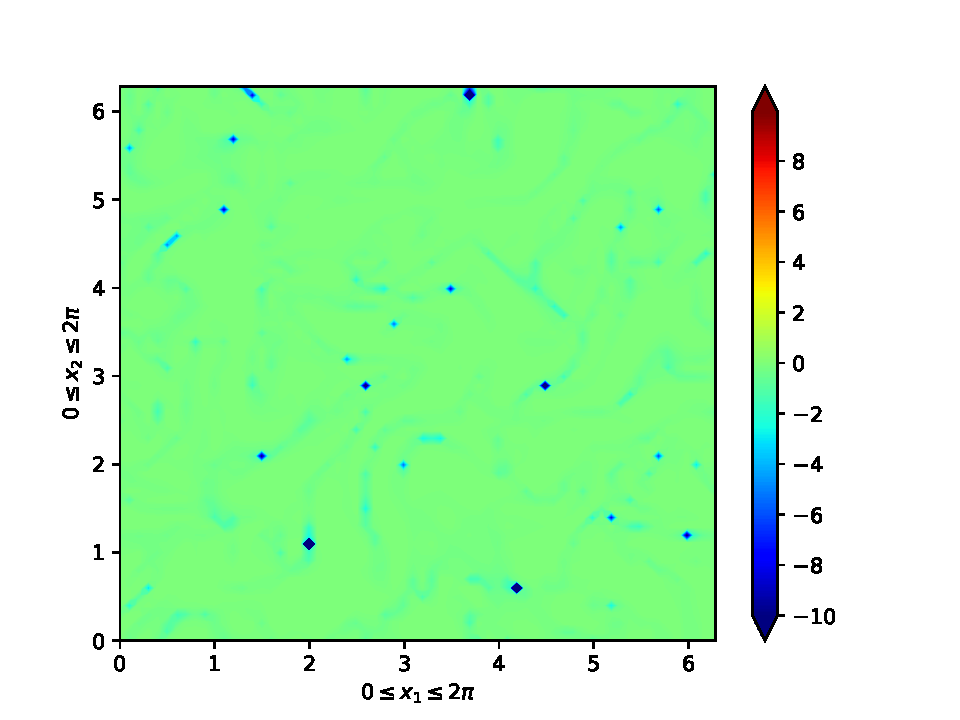
\includegraphics[height=1.75in]{media/run-cds-00/D-enst-CDS-00}
%        \caption{$D_{\Omega}$}
%    \end{subfigure}
%\end{figure}
%\newpage

%------------------------------------------------------------------------------%
% 1330                                                                         %
%------------------------------------------------------------------------------%
\begin{figure}[H]
    \begin{subfigure}[H]{0.45\textwidth}
        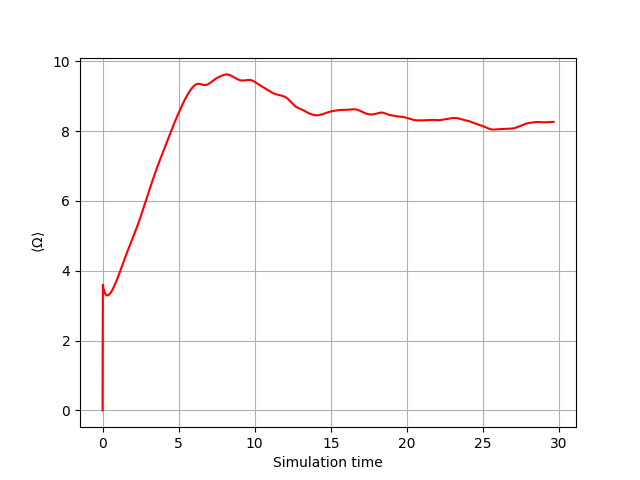
\includegraphics[height=1.75in]{media/run-cds-65/enst-average1330.png}
        \caption{Average enstrophy}
    \end{subfigure}
    ~
    \begin{subfigure}[H]{0.45\textwidth}
        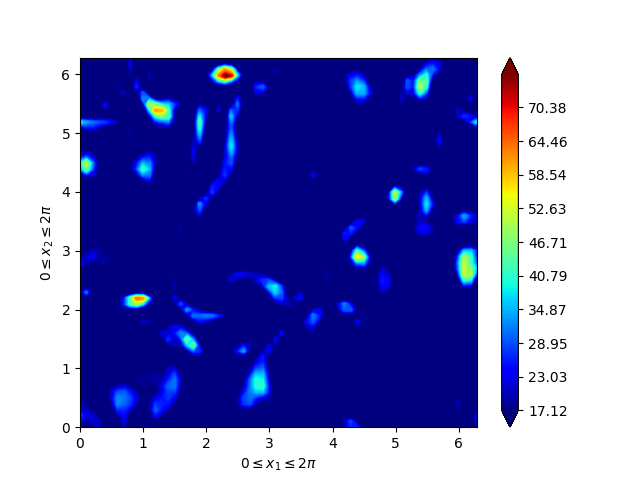
\includegraphics[height=1.75in]{media/run-cds-65/enst-2-1330.png}
        \caption{$[2\Omega_{rms}, \Omega_{max} ]$ }
    \end{subfigure}
    \newline
    \begin{subfigure}[H]{0.45\textwidth}
        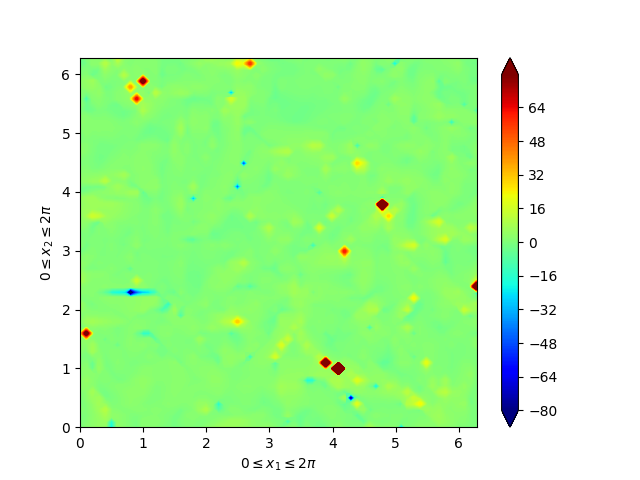
\includegraphics[height=1.75in]{media/run-cds-65/enst-1330.png}
        \caption{$\frac{1}{\Omega} \frac{D \Omega}{Dt}$}
    \end{subfigure}
    ~
    \begin{subfigure}{0.45\textwidth}
        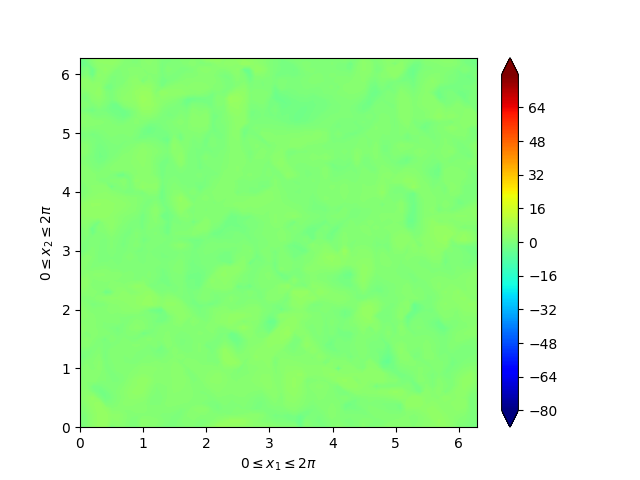
\includegraphics[height=1.75in]{media/run-cds-65/A-enst-1330.png}
        \caption{$A_{\Omega}$}
    \end{subfigure}
    \newline
    \begin{subfigure}{0.45\textwidth}
        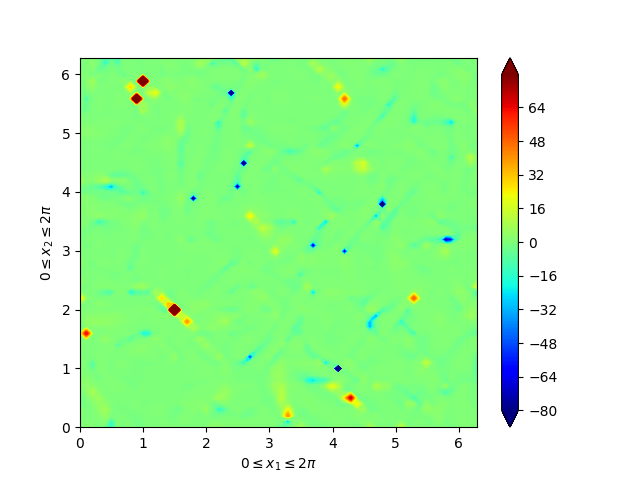
\includegraphics[height=1.75in]{media/run-cds-65/Pi-enst-1330.png}
        \caption{$C_{\Omega}$}
    \end{subfigure}
    ~
    \begin{subfigure}{0.45\textwidth}
        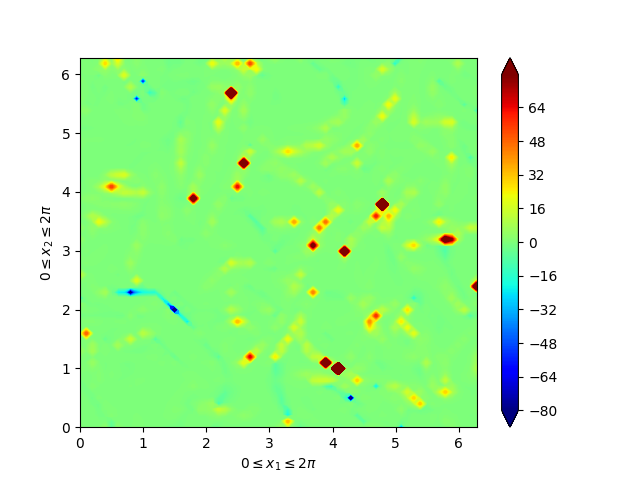
\includegraphics[height=1.75in]{media/run-cds-65/P-enst-1330.png}
        \caption{$P_{\Omega}$}
    \end{subfigure}
    \newline
    \begin{subfigure}{0.45\textwidth}
        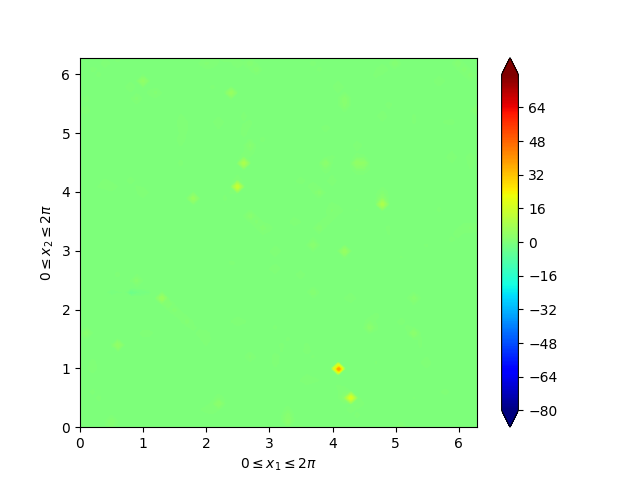
\includegraphics[height=1.75in]{media/run-cds-65/B-enst-1330.png}
        \caption{$B_{\Omega}$}
    \end{subfigure}
    ~
    \begin{subfigure}{0.45\textwidth}
        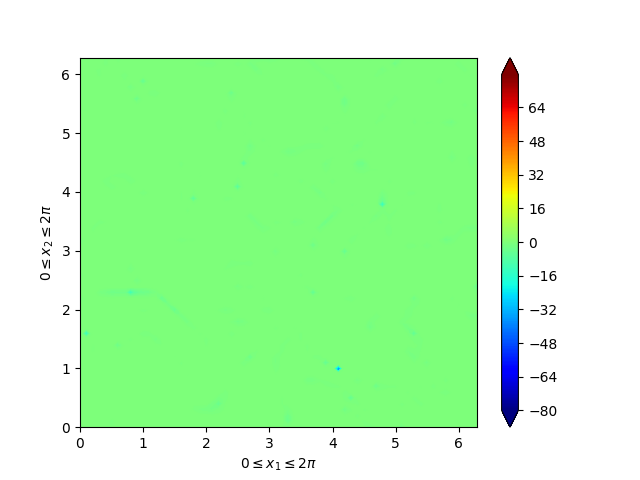
\includegraphics[height=1.75in]{media/run-cds-65/D-enst-1330.png}
        \caption{$D_{\Omega}$}
    \end{subfigure}
    \caption{Enstrophy transport terms for $t=29.65$, i.e., $t=t^{\ast} - 10 \Delta t$}
    \label{fig:enst-1330}
\end{figure}

\newpage

\begin{figure}[H]
    \begin{subfigure}[H]{0.45\textwidth}
        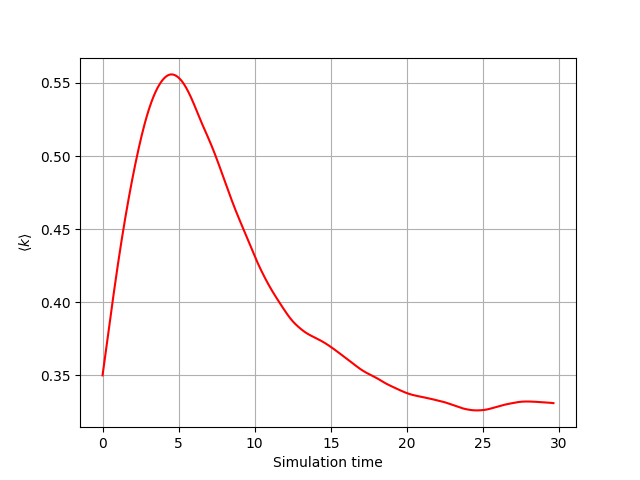
\includegraphics[height=1.75in]{media/run-cds-65/ke-average1330.png}
        \caption{Average kinetic energy}
    \end{subfigure}
    ~
    \begin{subfigure}[H]{0.45\textwidth}
        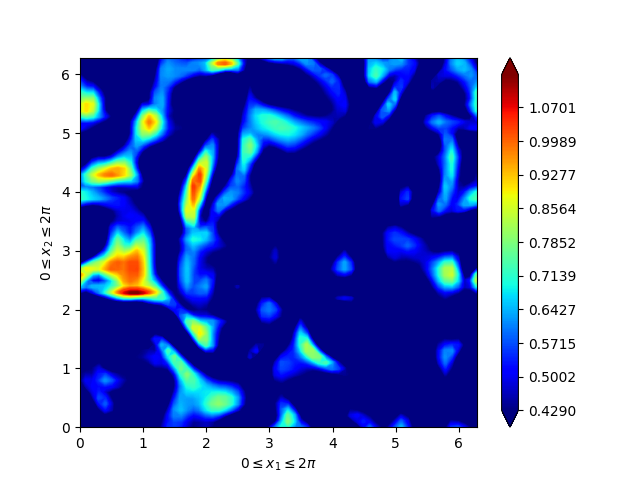
\includegraphics[height=1.75in]{media/run-cds-65/ke-2-1330.png}
        \caption{$[2k_{rms}, k_{max} $] }
    \end{subfigure}
    \newline
    \begin{subfigure}[H]{0.45\textwidth}
        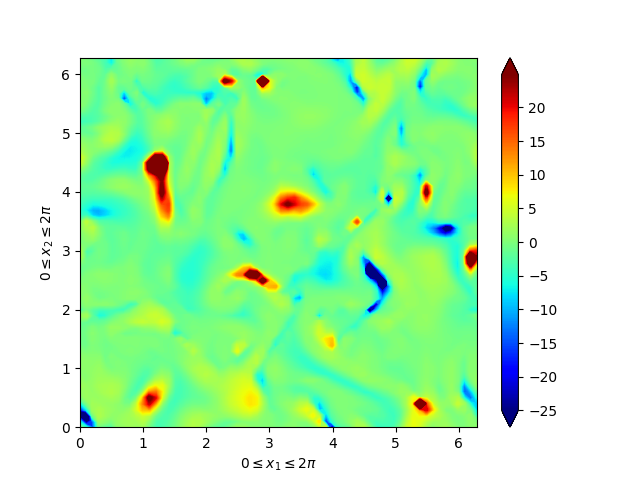
\includegraphics[height=1.75in]{media/run-cds-65/ke-1330.png}
        \caption{$\frac{1}{k} \frac{D k}{Dt}$}
    \end{subfigure}
    ~
    \begin{subfigure}{0.45\textwidth}
        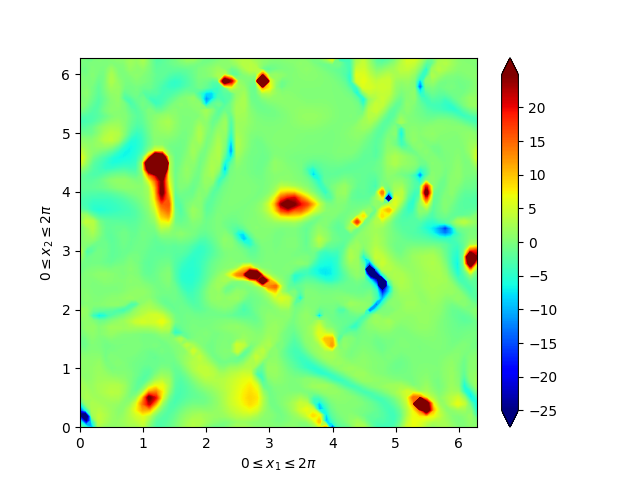
\includegraphics[height=1.75in]{media/run-cds-65/A-ke-1330.png}
        \caption{$A_{k}$}
    \end{subfigure}
    \newline
    \begin{subfigure}{0.45\textwidth}
        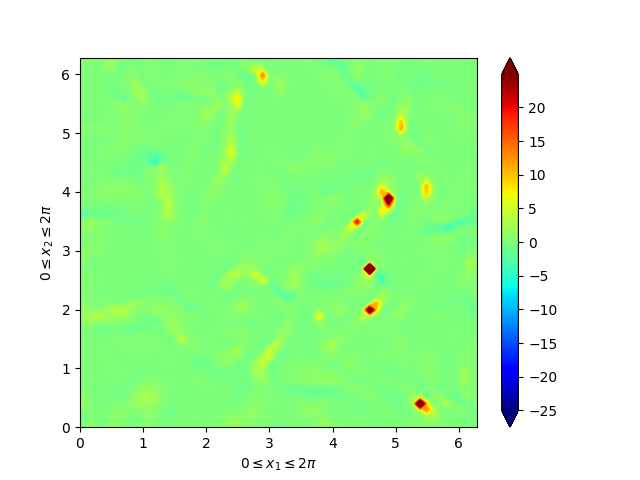
\includegraphics[height=1.75in]{media/run-cds-65/C-ke-1330.png}
        \caption{$C_{k}$}
    \end{subfigure}
    ~
    \begin{subfigure}{0.45\textwidth}
        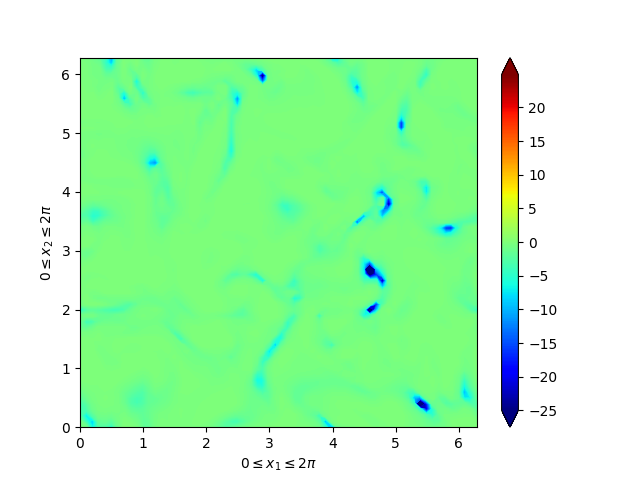
\includegraphics[height=1.75in]{media/run-cds-65/P-ke-1330.png}
        \caption{$P_{k}$}
    \end{subfigure}
    \newline
    \begin{subfigure}{0.45\textwidth}
        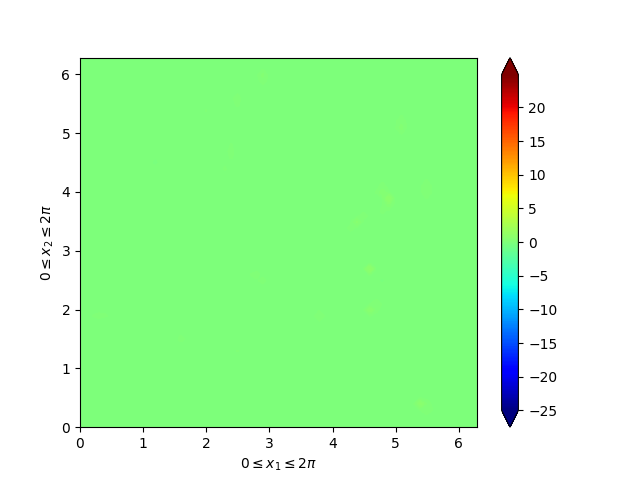
\includegraphics[height=1.75in]{media/run-cds-65/B-ke-1330.png}
        \caption{$B_{k}$}
    \end{subfigure}
    ~
    \begin{subfigure}{0.45\textwidth}
        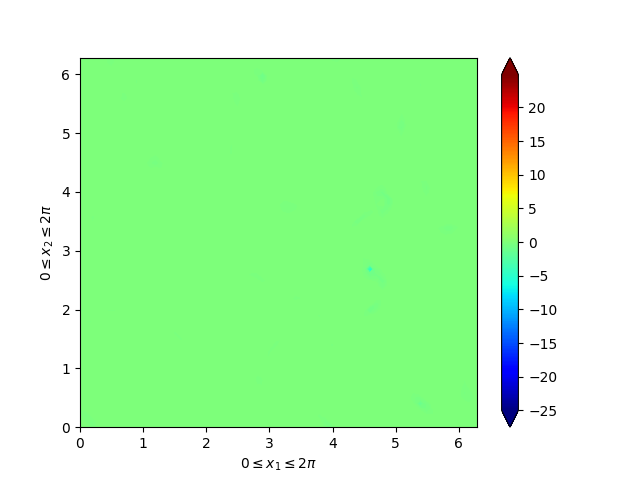
\includegraphics[height=1.75in]{media/run-cds-65/D-ke-1330.png}
        \caption{$D_{k}$}
    \end{subfigure}
    \caption{Kinetic energy transport terms for $t=29.65$, i.e., $t=t^{\ast} - 10 \Delta t$}
\end{figure}

\newpage

%------------------------------------------------------------------------------%
% 1335                                                                         %
%------------------------------------------------------------------------------%
\begin{figure}[H]
    \begin{subfigure}[H]{0.45\textwidth}
        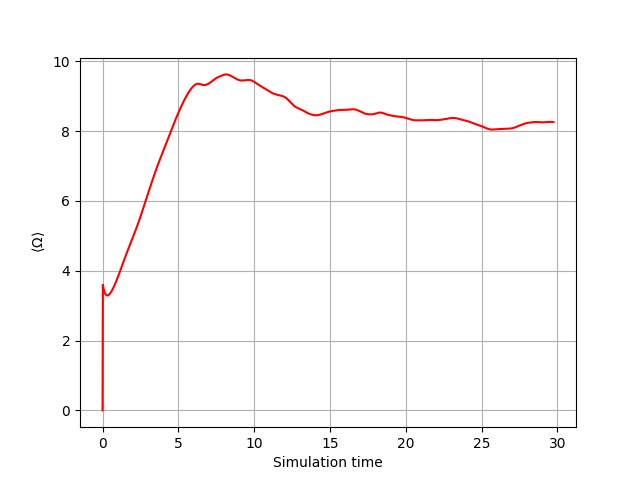
\includegraphics[height=1.75in]{media/run-cds-65/enst-average1335.png}
        \caption{Average enstrophy}
    \end{subfigure}
    ~
    \begin{subfigure}[H]{0.45\textwidth}
        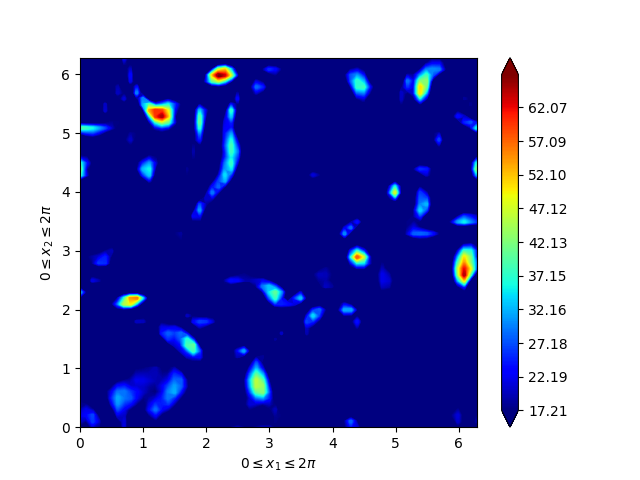
\includegraphics[height=1.75in]{media/run-cds-65/enst-2-1335.png}
        \caption{$[2\Omega_{rms}, \Omega_{max} $] }
    \end{subfigure}
    \newline
    \begin{subfigure}[H]{0.45\textwidth}
        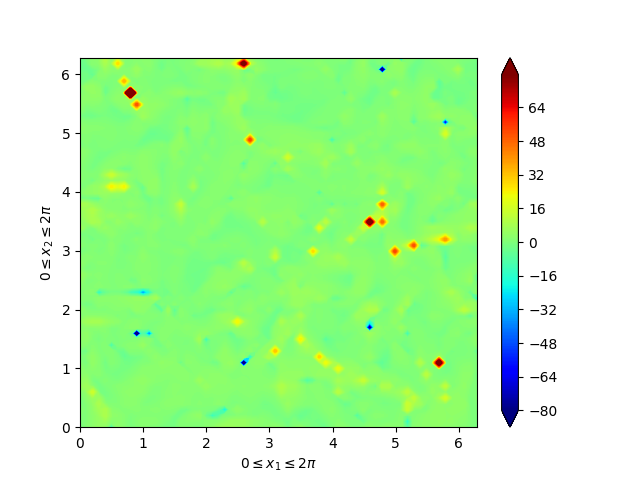
\includegraphics[height=1.75in]{media/run-cds-65/enst-1335.png}
        \caption{$\frac{1}{\Omega} \frac{D \Omega}{Dt}$}
    \end{subfigure}
    ~
    \begin{subfigure}{0.45\textwidth}
        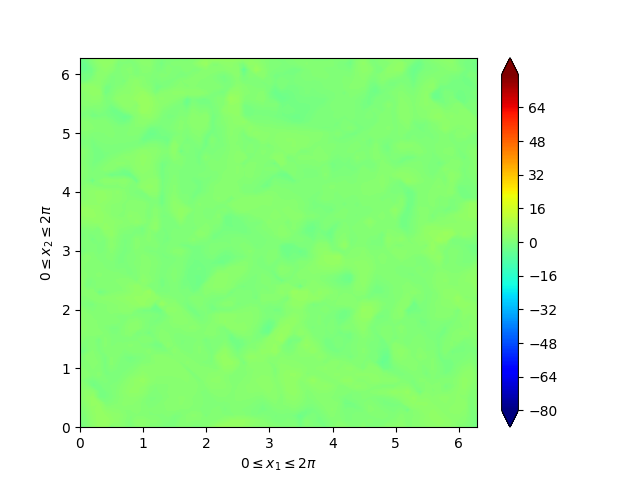
\includegraphics[height=1.75in]{media/run-cds-65/A-enst-1335.png}
        \caption{$A_{\Omega}$}
    \end{subfigure}
    \newline
    \begin{subfigure}{0.45\textwidth}
        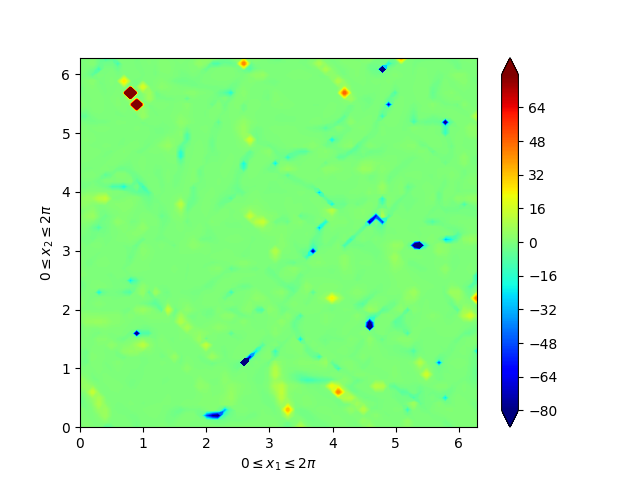
\includegraphics[height=1.75in]{media/run-cds-65/Pi-enst-1335.png}
        \caption{$C_{\Omega}$}
    \end{subfigure}
    ~
    \begin{subfigure}{0.45\textwidth}
        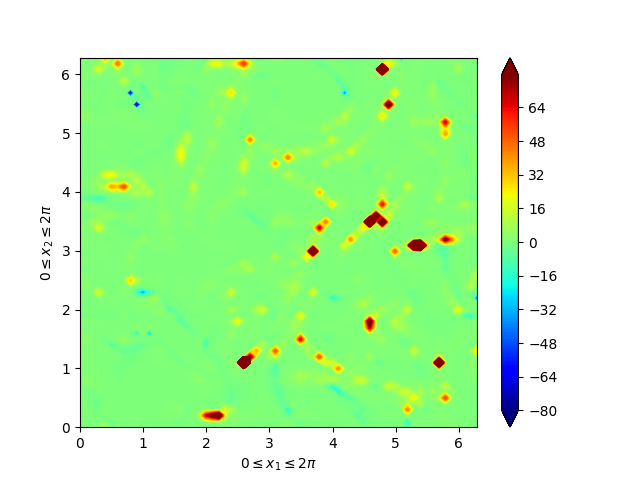
\includegraphics[height=1.75in]{media/run-cds-65/P-enst-1335.png}
        \caption{$P_{\Omega}$}
    \end{subfigure}
    \newline
    \begin{subfigure}{0.45\textwidth}
        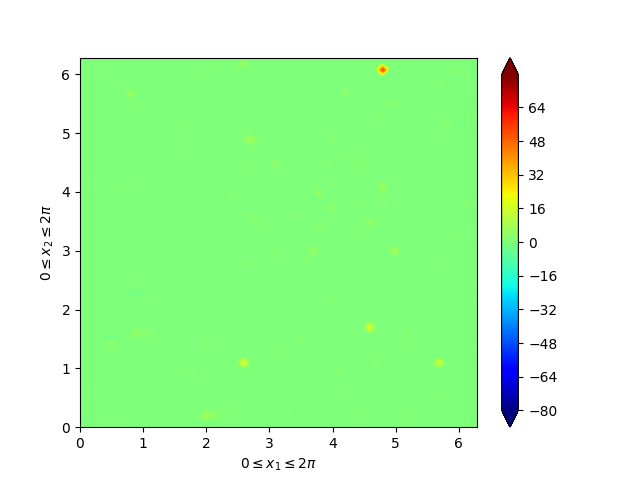
\includegraphics[height=1.75in]{media/run-cds-65/B-enst-1335.png}
        \caption{$B_{\Omega}$}
    \end{subfigure}
    ~
    \begin{subfigure}{0.45\textwidth}
        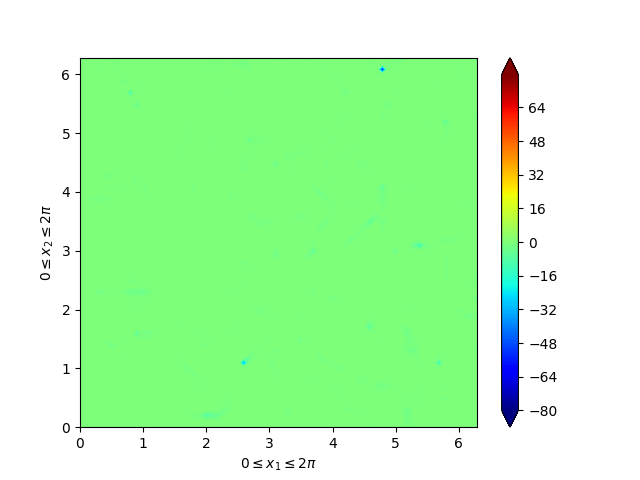
\includegraphics[height=1.75in]{media/run-cds-65/D-enst-1335.png}
        \caption{$D_{\Omega}$}
    \end{subfigure}
    \caption{Enstrophy transport terms for $t=29.77$, i.e., $t=t^{\ast} -5 \Delta t$}
\end{figure}

\newpage

\begin{figure}[H]
    \begin{subfigure}[H]{0.45\textwidth}
        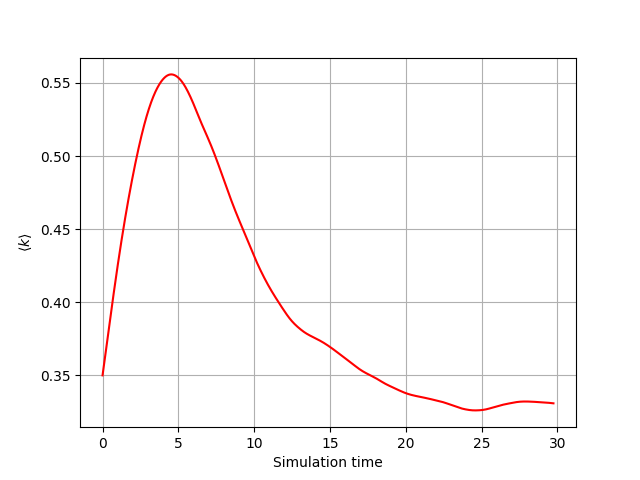
\includegraphics[height=1.75in]{media/run-cds-65/ke-average1335.png}
        \caption{Average kinetic energy}
    \end{subfigure}
    ~
    \begin{subfigure}[H]{0.45\textwidth}
        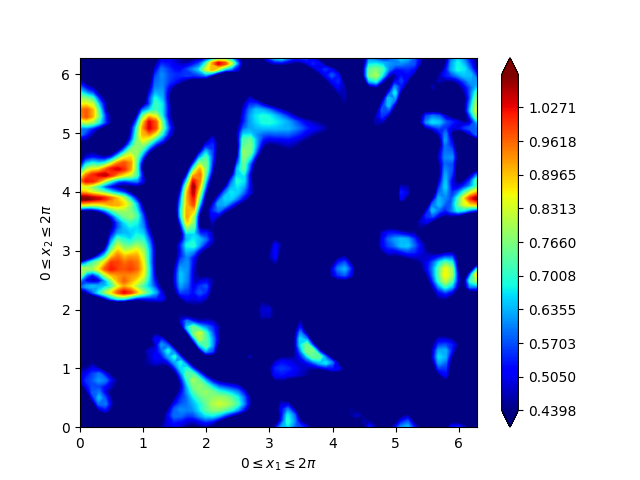
\includegraphics[height=1.75in]{media/run-cds-65/ke-2-1335.png}
        \caption{$[2k_{rms}, k_{max} $] }
    \end{subfigure}
    \newline
    \begin{subfigure}[H]{0.45\textwidth}
        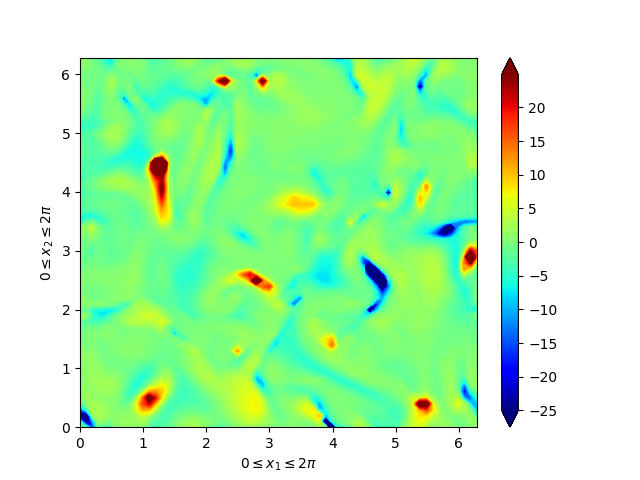
\includegraphics[height=1.75in]{media/run-cds-65/ke-1335.png}
        \caption{$\frac{1}{k} \frac{D k}{Dt}$}
    \end{subfigure}
    ~
    \begin{subfigure}{0.45\textwidth}
        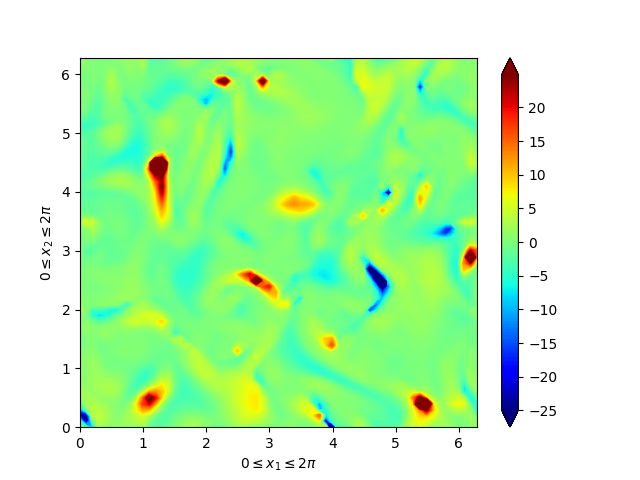
\includegraphics[height=1.75in]{media/run-cds-65/A-ke-1335.png}
        \caption{$A_{k}$}
    \end{subfigure}
    \newline
    \begin{subfigure}{0.45\textwidth}
        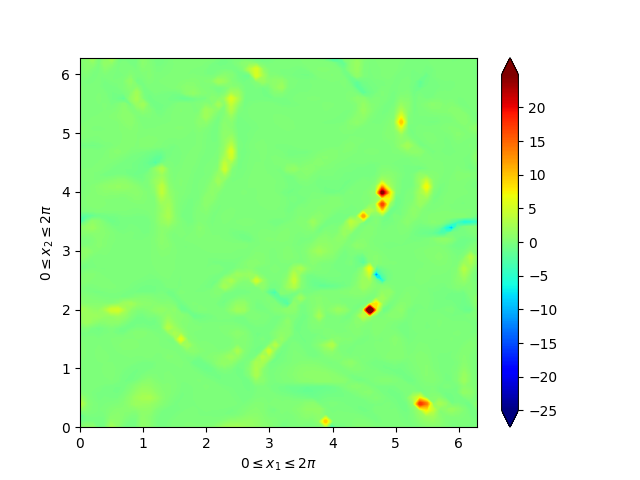
\includegraphics[height=1.75in]{media/run-cds-65/C-ke-1335.png}
        \caption{$C_{k}$}
    \end{subfigure}
    ~
    \begin{subfigure}{0.45\textwidth}
        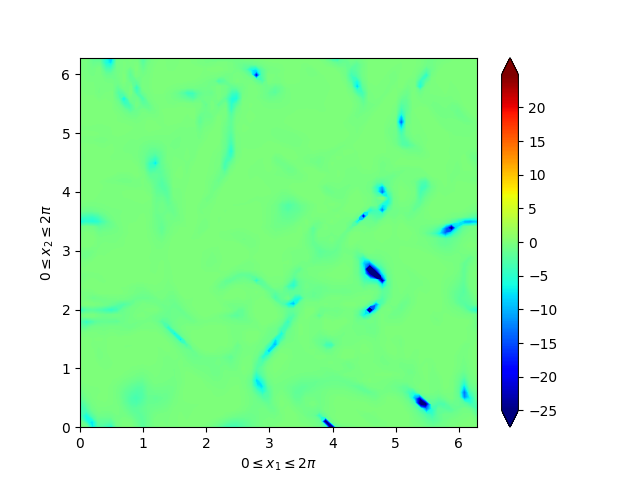
\includegraphics[height=1.75in]{media/run-cds-65/P-ke-1335.png}
        \caption{$P_{k}$}
    \end{subfigure}
    \newline
    \begin{subfigure}{0.45\textwidth}
        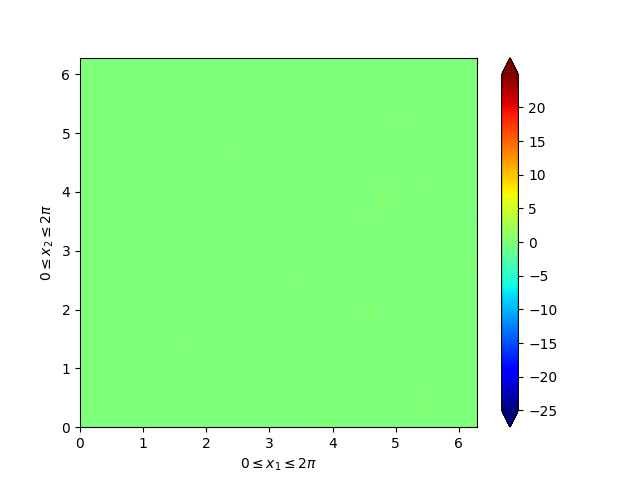
\includegraphics[height=1.75in]{media/run-cds-65/B-ke-1335.png}
        \caption{$B_{k}$}
    \end{subfigure}
    ~
    \begin{subfigure}{0.45\textwidth}
        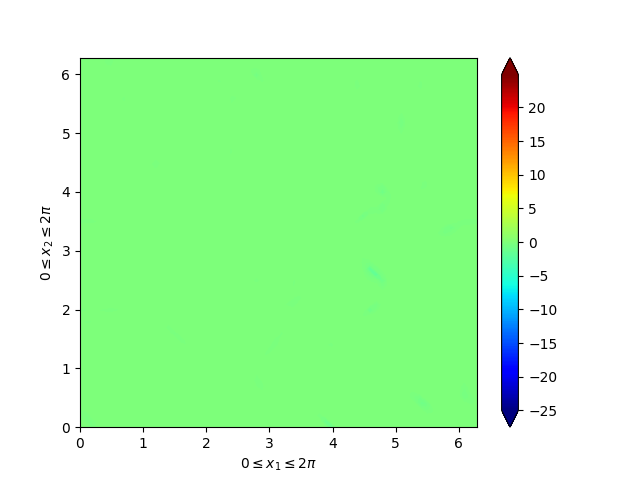
\includegraphics[height=1.75in]{media/run-cds-65/D-ke-1335.png}
        \caption{$D_{k}$}
    \end{subfigure}
    \caption{Kinetic energy transport terms for $t=29.77$, i.e., $t=t^{\ast} -5 \Delta t$}
\end{figure}

%------------------------------------------------------------------------------%
% 1340                                                                         %
%------------------------------------------------------------------------------%
\begin{figure}[H]
    \begin{subfigure}[H]{0.45\textwidth}
        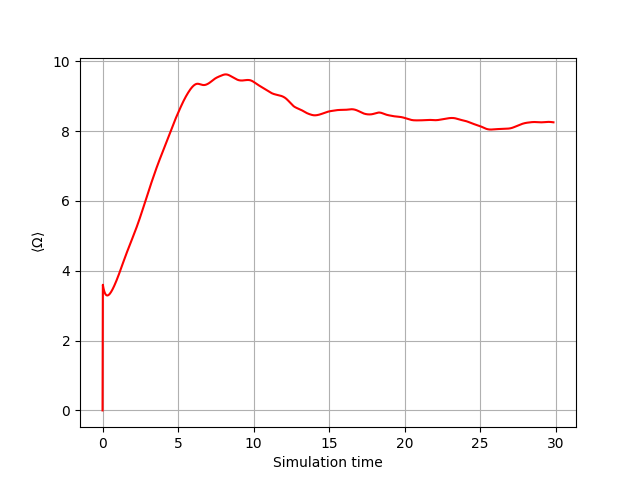
\includegraphics[height=1.75in]{media/run-cds-65/enst-average1340.png}
        \caption{Average enstrophy}
    \end{subfigure}
    ~
    \begin{subfigure}[H]{0.45\textwidth}
        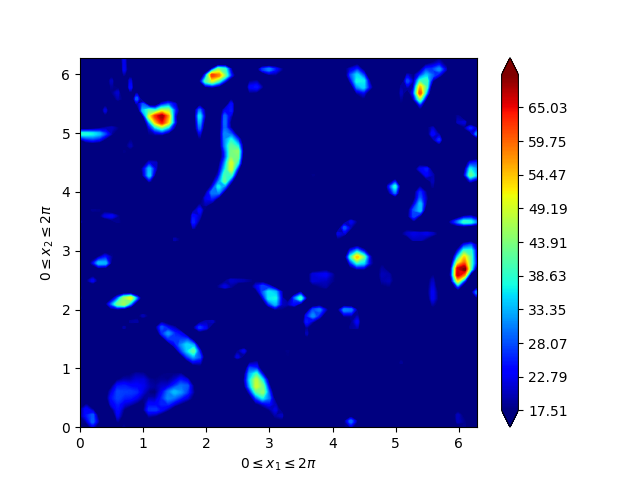
\includegraphics[height=1.75in]{media/run-cds-65/enst-2-1340.png}
        \caption{$[2\Omega_{rms}, \Omega_{max} $] }
    \end{subfigure}
    \newline
    \begin{subfigure}[H]{0.45\textwidth}
        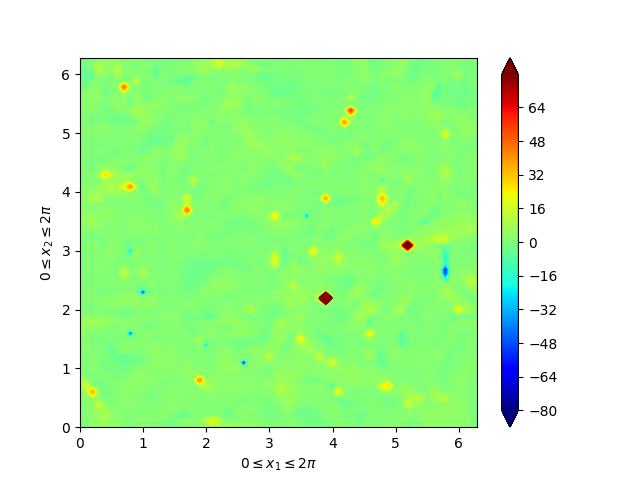
\includegraphics[height=1.75in]{media/run-cds-65/enst-1340.png}
        \caption{$\frac{1}{\Omega} \frac{D \Omega}{Dt}$}
    \end{subfigure}
    ~
    \begin{subfigure}{0.45\textwidth}
        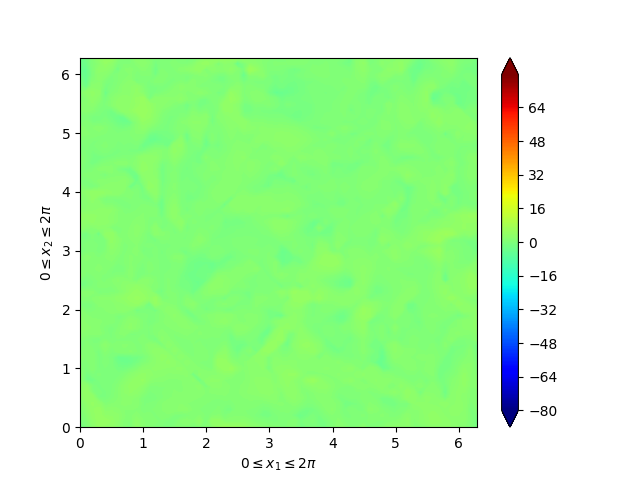
\includegraphics[height=1.75in]{media/run-cds-65/A-enst-1340.png}
        \caption{$A_{\Omega}$}
    \end{subfigure}
    \newline
    \begin{subfigure}{0.45\textwidth}
        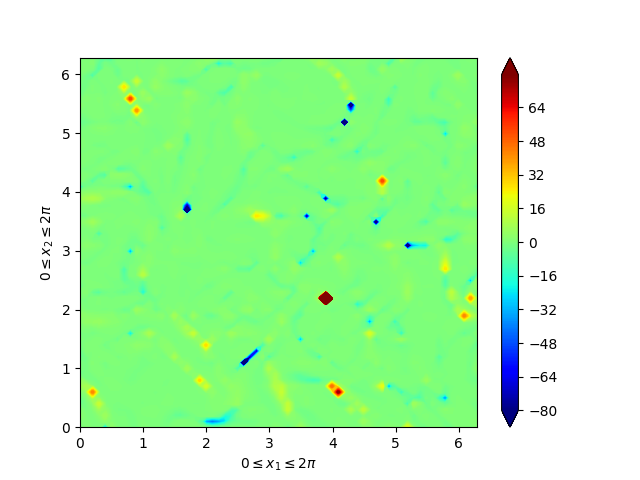
\includegraphics[height=1.75in]{media/run-cds-65/Pi-enst-1340.png}
        \caption{$C_{\Omega}$}
    \end{subfigure}
    ~
    \begin{subfigure}{0.45\textwidth}
        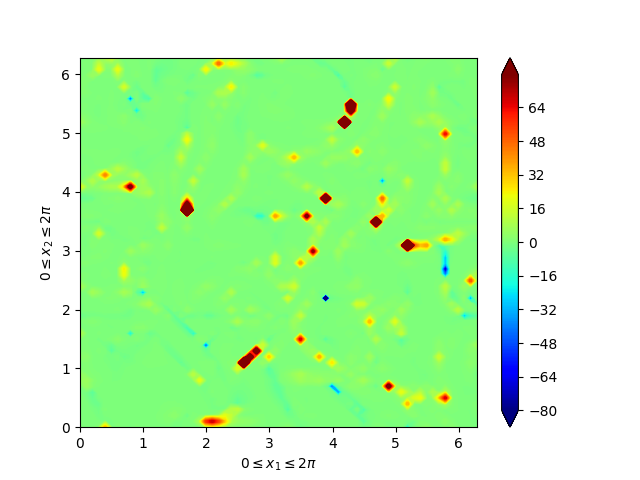
\includegraphics[height=1.75in]{media/run-cds-65/P-enst-1340.png}
        \caption{$P_{\Omega}$}
    \end{subfigure}
    \newline
    \begin{subfigure}{0.45\textwidth}
        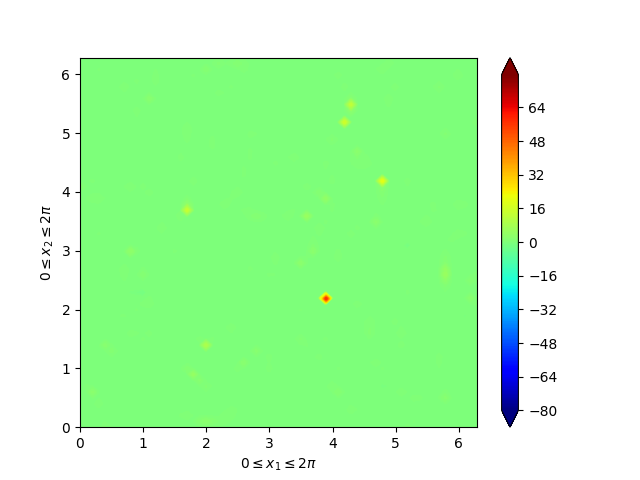
\includegraphics[height=1.75in]{media/run-cds-65/B-enst-1340.png}
        \caption{$B_{\Omega}$}
    \end{subfigure}
    ~
    \begin{subfigure}{0.45\textwidth}
        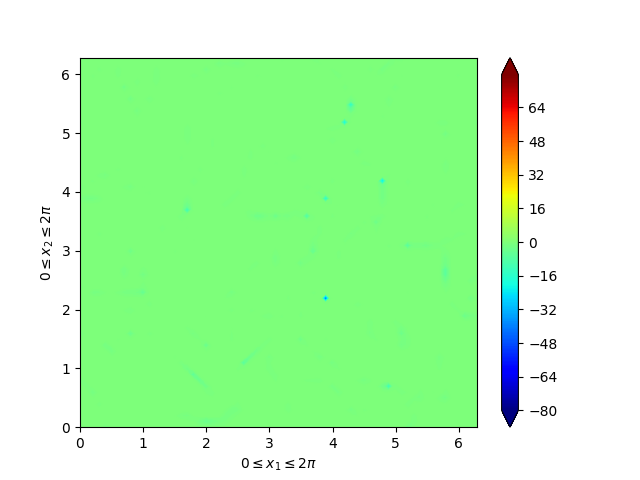
\includegraphics[height=1.75in]{media/run-cds-65/D-enst-1340.png}
        \caption{$D_{\Omega}$}
    \end{subfigure}
    \caption{Enstrophy transport terms for $t=30.01$, i.e., $t=t^{\ast} $}
\end{figure}

\newpage

\begin{figure}[H]
    \begin{subfigure}[H]{0.45\textwidth}
        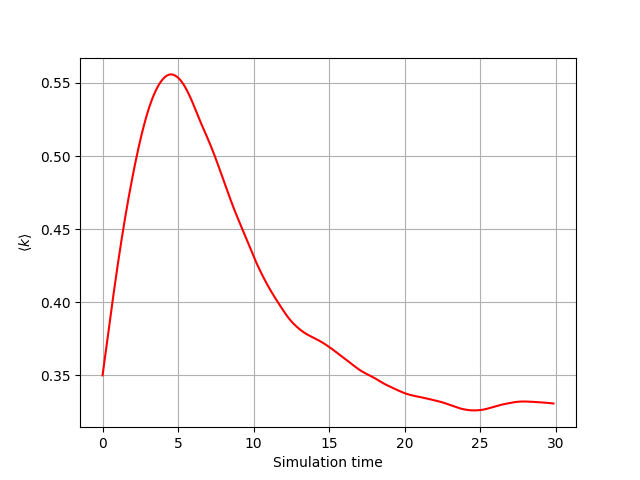
\includegraphics[height=1.75in]{media/run-cds-65/ke-average1340.png}
        \caption{Average kinetic energy}
    \end{subfigure}
    ~
    \begin{subfigure}[H]{0.45\textwidth}
        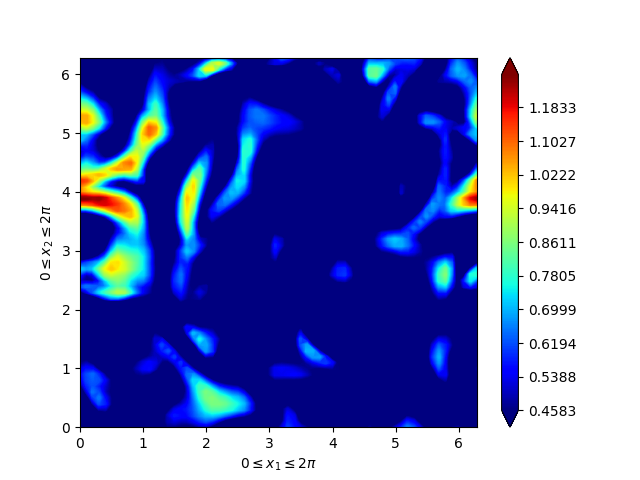
\includegraphics[height=1.75in]{media/run-cds-65/ke-2-1340.png}
        \caption{$[2k_{rms}, k_{max} $] }
    \end{subfigure}
    \newline
    \begin{subfigure}[H]{0.45\textwidth}
        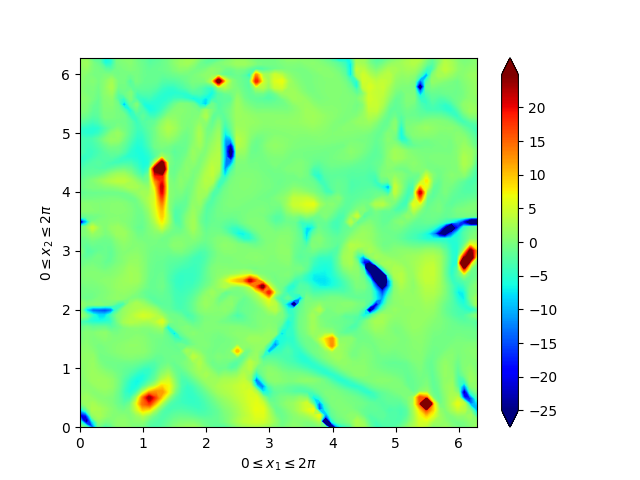
\includegraphics[height=1.75in]{media/run-cds-65/ke-1340.png}
        \caption{$\frac{1}{k} \frac{D k}{Dt}$}
    \end{subfigure}
    ~
    \begin{subfigure}{0.45\textwidth}
        \includegraphics[height=1.75in]{media/run-cds-65/A-ke-1340.png}
        \caption{$A_{k}$}
    \end{subfigure}
    \newline
    \begin{subfigure}{0.45\textwidth}
        \includegraphics[height=1.75in]{media/run-cds-65/C-ke-1340.png}
        \caption{$C_{k}$}
    \end{subfigure}
    ~
    \begin{subfigure}{0.45\textwidth}
        \includegraphics[height=1.75in]{media/run-cds-65/P-ke-1340.png}
        \caption{$P_{k}$}
    \end{subfigure}
    \newline
    \begin{subfigure}{0.45\textwidth}
        \includegraphics[height=1.75in]{media/run-cds-65/B-ke-1340.png}
        \caption{$B_{k}$}
    \end{subfigure}
    ~
    \begin{subfigure}{0.45\textwidth}
        \includegraphics[height=1.75in]{media/run-cds-65/D-ke-1340.png}
        \caption{$D_{k}$}
    \end{subfigure}
    \caption{Kinetic energy transport terms for $t=30.01$, i.e., $t=t^{\ast} $}
\end{figure}
%------------------------------------------------------------------------------%
% 1360                                                                         %
%------------------------------------------------------------------------------%
\begin{figure}[H]
    \begin{subfigure}[H]{0.45\textwidth}
        \includegraphics[height=1.75in]{media/run-cds-65/enst-average1360.png}
        \caption{Average enstrophy}
    \end{subfigure}
    ~
    \begin{subfigure}[H]{0.45\textwidth}
        \includegraphics[height=1.75in]{media/run-cds-65/enst-2-1360.png}
        \caption{$[2\Omega_{rms}, \Omega_{max} $] }
    \end{subfigure}
    \newline
    \begin{subfigure}[H]{0.45\textwidth}
        \includegraphics[height=1.75in]{media/run-cds-65/enst-1360.png}
        \caption{$\frac{1}{\Omega} \frac{D \Omega}{Dt}$}
    \end{subfigure}
    ~
    \begin{subfigure}{0.45\textwidth}
        \includegraphics[height=1.75in]{media/run-cds-65/A-enst-1360.png}
        \caption{$A_{\Omega}$}
    \end{subfigure}
    \newline
    \begin{subfigure}{0.45\textwidth}
        \includegraphics[height=1.75in]{media/run-cds-65/Pi-enst-1360.png}
        \caption{$C_{\Omega}$}
    \end{subfigure}
    ~
    \begin{subfigure}{0.45\textwidth}
        \includegraphics[height=1.75in]{media/run-cds-65/P-enst-1360.png}
        \caption{$P_{\Omega}$}
    \end{subfigure}
    \newline
    \begin{subfigure}{0.45\textwidth}
        \includegraphics[height=1.75in]{media/run-cds-65/B-enst-1360.png}
        \caption{$B_{\Omega}$}
    \end{subfigure}
    ~
    \begin{subfigure}{0.45\textwidth}
        \includegraphics[height=1.75in]{media/run-cds-65/D-enst-1360.png}
        \caption{$D_{\Omega}$}
    \end{subfigure}
    \caption{Enstrophy transport terms for $t=30.32$, i.e., $t=t^{\ast} + 20 \Delta t$}
\end{figure}

\newpage

\begin{figure}[H]
    \begin{subfigure}[H]{0.45\textwidth}
        \includegraphics[height=1.75in]{media/run-cds-65/ke-average1360.png}
        \caption{Average kinetic energy}
    \end{subfigure}
    ~
    \begin{subfigure}[H]{0.45\textwidth}
        \includegraphics[height=1.75in]{media/run-cds-65/ke-2-1360.png}
        \caption{$[2k_{rms}, k_{max} $] }
    \end{subfigure}
    \newline
    \begin{subfigure}[H]{0.45\textwidth}
        \includegraphics[height=1.75in]{media/run-cds-65/ke-1360.png}
        \caption{$\frac{1}{k} \frac{D k}{Dt}$}
    \end{subfigure}
    ~
    \begin{subfigure}{0.45\textwidth}
        \includegraphics[height=1.75in]{media/run-cds-65/A-ke-1360.png}
        \caption{$A_{k}$}
    \end{subfigure}
    \newline
    \begin{subfigure}{0.45\textwidth}
        \includegraphics[height=1.75in]{media/run-cds-65/C-ke-1360.png}
        \caption{$C_{k}$}
    \end{subfigure}
    ~
    \begin{subfigure}{0.45\textwidth}
        \includegraphics[height=1.75in]{media/run-cds-65/P-ke-1360.png}
        \caption{$P_{k}$}
    \end{subfigure}
    \newline
    \begin{subfigure}{0.45\textwidth}
        \includegraphics[height=1.75in]{media/run-cds-65/B-ke-1360.png}
        \caption{$B_{k}$}
    \end{subfigure}
    ~
    \begin{subfigure}{0.45\textwidth}
        \includegraphics[height=1.75in]{media/run-cds-65/D-ke-1360.png}
        \caption{$D_{k}$}
    \end{subfigure}
    \caption{Kinetic energy transport terms for $t=30.32$, i.e., $t=t^{\ast} + 20 \Delta t$}
\end{figure}

%------------------------------------------------------------------------------%
% 1380                                                                         %
%------------------------------------------------------------------------------%
\begin{figure}[H]
    \begin{subfigure}[H]{0.45\textwidth}
        \includegraphics[height=1.75in]{media/run-cds-65/enst-average1380.png}
        \caption{Average enstrophy}
    \end{subfigure}
    ~
    \begin{subfigure}[H]{0.45\textwidth}
        \includegraphics[height=1.75in]{media/run-cds-65/enst-2-1380.png}
        \caption{$[2\Omega_{rms}, \Omega_{max} $] }
    \end{subfigure}
    \newline
    \begin{subfigure}[H]{0.45\textwidth}
        \includegraphics[height=1.75in]{media/run-cds-65/enst-1380.png}
        \caption{$\frac{1}{\Omega} \frac{D \Omega}{Dt}$}
    \end{subfigure}
    ~
    \begin{subfigure}{0.45\textwidth}
        \includegraphics[height=1.75in]{media/run-cds-65/A-enst-1380.png}
        \caption{$A_{\Omega}$}
    \end{subfigure}
    \newline
    \begin{subfigure}{0.45\textwidth}
        \includegraphics[height=1.75in]{media/run-cds-65/Pi-enst-1380.png}
        \caption{$C_{\Omega}$}
    \end{subfigure}
    ~
    \begin{subfigure}{0.45\textwidth}
        \includegraphics[height=1.75in]{media/run-cds-65/P-enst-1380.png}
        \caption{$P_{\Omega}$}
    \end{subfigure}
    \newline
    \begin{subfigure}{0.45\textwidth}
        \includegraphics[height=1.75in]{media/run-cds-65/B-enst-1380.png}
        \caption{$B_{\Omega}$}
    \end{subfigure}
    ~
    \begin{subfigure}{0.45\textwidth}
        \includegraphics[height=1.75in]{media/run-cds-65/D-enst-1380.png}
        \caption{$D_{\Omega}$}
    \end{subfigure}
    \caption{Enstrophy transport terms for $t=30.67$, i.e., $t=t^{\ast} + 40 \Delta t$}
\end{figure}

\newpage

\begin{figure}[H]
    \begin{subfigure}[H]{0.45\textwidth}
        \includegraphics[height=1.75in]{media/run-cds-65/ke-average1380.png}
        \caption{Average kinetic energy}
    \end{subfigure}
    ~
    \begin{subfigure}[H]{0.45\textwidth}
        \includegraphics[height=1.75in]{media/run-cds-65/ke-2-1380.png}
        \caption{$[2k_{rms}, k_{max} $] }
    \end{subfigure}
    \newline
    \begin{subfigure}[H]{0.45\textwidth}
        \includegraphics[height=1.75in]{media/run-cds-65/ke-1380.png}
        \caption{$\frac{1}{k} \frac{D k}{Dt}$}
    \end{subfigure}
    ~
    \begin{subfigure}{0.45\textwidth}
        \includegraphics[height=1.75in]{media/run-cds-65/A-ke-1380.png}
        \caption{$A_{k}$}
    \end{subfigure}
    \newline
    \begin{subfigure}{0.45\textwidth}
        \includegraphics[height=1.75in]{media/run-cds-65/C-ke-1380.png}
        \caption{$C_{k}$}
    \end{subfigure}
    ~
    \begin{subfigure}{0.45\textwidth}
        \includegraphics[height=1.75in]{media/run-cds-65/P-ke-1380.png}
        \caption{$P_{k}$}
    \end{subfigure}
    \newline
    \begin{subfigure}{0.45\textwidth}
        \includegraphics[height=1.75in]{media/run-cds-65/B-ke-1380.png}
        \caption{$B_{k}$}
    \end{subfigure}
    ~
    \begin{subfigure}{0.45\textwidth}
        \includegraphics[height=1.75in]{media/run-cds-65/D-ke-1380.png}
        \caption{$D_{k}$}
    \end{subfigure}
    \caption{Kinetic energy transport terms for $t=30.67$, i.e., $t=t^{\ast} + 40 \Delta t$}
\end{figure}
%------------------------------------------------------------------------------%
% 1400                                                                         %
%------------------------------------------------------------------------------%
\begin{figure}[H]
    \begin{subfigure}[H]{0.45\textwidth}
        \includegraphics[height=1.75in]{media/run-cds-65/enst-average1400.png}
        \caption{Average enstrophy}
    \end{subfigure}
    ~
    \begin{subfigure}[H]{0.45\textwidth}
        \includegraphics[height=1.75in]{media/run-cds-65/enst-2-1400.png}
        \caption{$[2\Omega_{rms}, \Omega_{max} $] }
    \end{subfigure}
    \newline
    \begin{subfigure}[H]{0.45\textwidth}
        \includegraphics[height=1.75in]{media/run-cds-65/enst-1400.png}
        \caption{$\frac{1}{\Omega} \frac{D \Omega}{Dt}$}
    \end{subfigure}
    ~
    \begin{subfigure}{0.45\textwidth}
        \includegraphics[height=1.75in]{media/run-cds-65/A-enst-1400.png}
        \caption{$A_{\Omega}$}
    \end{subfigure}
    \newline
    \begin{subfigure}{0.45\textwidth}
        \includegraphics[height=1.75in]{media/run-cds-65/Pi-enst-1400.png}
        \caption{$C_{\Omega}$}
    \end{subfigure}
    ~
    \begin{subfigure}{0.45\textwidth}
        \includegraphics[height=1.75in]{media/run-cds-65/P-enst-1400.png}
        \caption{$P_{\Omega}$}
    \end{subfigure}
    \newline
    \begin{subfigure}{0.45\textwidth}
        \includegraphics[height=1.75in]{media/run-cds-65/B-enst-1400.png}
        \caption{$B_{\Omega}$}
    \end{subfigure}
    ~
    \begin{subfigure}{0.45\textwidth}
        \includegraphics[height=1.75in]{media/run-cds-65/D-enst-1400.png}
        \caption{$D_{\Omega}$}
    \end{subfigure}
    \caption{Enstrophy transport terms for $t=30.80$, i.e., $t=t^{\ast} + 60 \Delta t$}
\end{figure}

\newpage

\begin{figure}[H]
    \begin{subfigure}[H]{0.45\textwidth}
        \includegraphics[height=1.75in]{media/run-cds-65/ke-average1400.png}
        \caption{Average kinetic energy}
    \end{subfigure}
    ~
    \begin{subfigure}[H]{0.45\textwidth}
        \includegraphics[height=1.75in]{media/run-cds-65/ke-2-1400.png}
        \caption{$[2k_{rms}, k_{max} $] }
    \end{subfigure}
    \newline
    \begin{subfigure}[H]{0.45\textwidth}
        \includegraphics[height=1.75in]{media/run-cds-65/ke-1400.png}
        \caption{$\frac{1}{k} \frac{D k}{Dt}$}
    \end{subfigure}
    ~
    \begin{subfigure}{0.45\textwidth}
        \includegraphics[height=1.75in]{media/run-cds-65/A-ke-1400.png}
        \caption{$A_{k}$}
    \end{subfigure}
    \newline
    \begin{subfigure}{0.45\textwidth}
        \includegraphics[height=1.75in]{media/run-cds-65/C-ke-1400.png}
        \caption{$C_{k}$}
    \end{subfigure}
    ~
    \begin{subfigure}{0.45\textwidth}
        \includegraphics[height=1.75in]{media/run-cds-65/P-ke-1400.png}
        \caption{$P_{k}$}
    \end{subfigure}
    \newline
    \begin{subfigure}{0.45\textwidth}
        \includegraphics[height=1.75in]{media/run-cds-65/B-ke-1400.png}
        \caption{$B_{k}$}
    \end{subfigure}
    ~
    \begin{subfigure}{0.45\textwidth}
        \includegraphics[height=1.75in]{media/run-cds-65/D-ke-1400.png}
        \caption{$D_{k}$}
    \end{subfigure}
    \caption{Kinetic energy transport terms for $t=30.80$, i.e., $t=t^{\ast} + 60 \Delta t$}
\end{figure}
%------------------------------------------------------------------------------%
% 1420                                                                         %
%------------------------------------------------------------------------------%
\begin{figure}[H]
    \begin{subfigure}[H]{0.45\textwidth}
        \includegraphics[height=1.75in]{media/run-cds-65/enst-average1420.png}
        \caption{Average enstrophy}
    \end{subfigure}
    ~
    \begin{subfigure}[H]{0.45\textwidth}
        \includegraphics[height=1.75in]{media/run-cds-65/enst-2-1420.png}
        \caption{$[2\Omega_{rms}, \Omega_{max} $] }
    \end{subfigure}
    \newline
    \begin{subfigure}[H]{0.45\textwidth}
        \includegraphics[height=1.75in]{media/run-cds-65/enst-1420.png}
        \caption{$\frac{1}{\Omega} \frac{D \Omega}{Dt}$}
    \end{subfigure}
    ~
    \begin{subfigure}{0.45\textwidth}
        \includegraphics[height=1.75in]{media/run-cds-65/A-enst-1420.png}
        \caption{$A_{\Omega}$}
    \end{subfigure}
    \newline
    \begin{subfigure}{0.45\textwidth}
        \includegraphics[height=1.75in]{media/run-cds-65/Pi-enst-1420.png}
        \caption{$C_{\Omega}$}
    \end{subfigure}
    ~
    \begin{subfigure}{0.45\textwidth}
        \includegraphics[height=1.75in]{media/run-cds-65/P-enst-1420.png}
        \caption{$P_{\Omega}$}
    \end{subfigure}
    \newline
    \begin{subfigure}{0.45\textwidth}
        \includegraphics[height=1.75in]{media/run-cds-65/B-enst-1420.png}
        \caption{$B_{\Omega}$}
    \end{subfigure}
    ~
    \begin{subfigure}{0.45\textwidth}
        \includegraphics[height=1.75in]{media/run-cds-65/D-enst-1420.png}
        \caption{$D_{\Omega}$}
    \end{subfigure}
    \caption{Enstrophy transport terms for $t=30.88$, i.e., $t=t^{\ast} + 80 \Delta t$}
\end{figure}

\newpage

\begin{figure}[H]
    \begin{subfigure}[H]{0.45\textwidth}
        \includegraphics[height=1.75in]{media/run-cds-65/ke-average1420.png}
        \caption{Average kinetic energy}
    \end{subfigure}
    ~
    \begin{subfigure}[H]{0.45\textwidth}
        \includegraphics[height=1.75in]{media/run-cds-65/ke-2-1420.png}
        \caption{$[2k_{rms}, k_{max} $] }
    \end{subfigure}
    \newline
    \begin{subfigure}[H]{0.45\textwidth}
        \includegraphics[height=1.75in]{media/run-cds-65/ke-1420.png}
        \caption{$\frac{1}{k} \frac{D k}{Dt}$}
    \end{subfigure}
    ~
    \begin{subfigure}{0.45\textwidth}
        \includegraphics[height=1.75in]{media/run-cds-65/A-ke-1420.png}
        \caption{$A_{k}$}
    \end{subfigure}
    \newline
    \begin{subfigure}{0.45\textwidth}
        \includegraphics[height=1.75in]{media/run-cds-65/C-ke-1420.png}
        \caption{$C_{k}$}
    \end{subfigure}
    ~
    \begin{subfigure}{0.45\textwidth}
        \includegraphics[height=1.75in]{media/run-cds-65/P-ke-1420.png}
        \caption{$P_{k}$}
    \end{subfigure}
    \newline
    \begin{subfigure}{0.45\textwidth}
        \includegraphics[height=1.75in]{media/run-cds-65/B-ke-1420.png}
        \caption{$B_{k}$}
    \end{subfigure}
    ~
    \begin{subfigure}{0.45\textwidth}
        \includegraphics[height=1.75in]{media/run-cds-65/D-ke-1420.png}
        \caption{$D_{k}$}
    \end{subfigure}
    \caption{Kinetic energy transport terms for $t=30.88$, i.e., $t=t^{\ast} + 80 \Delta t$}
\end{figure}
%------------------------------------------------------------------------------%
% 1440                                                                         %
%------------------------------------------------------------------------------%
\begin{figure}[H]
    \begin{subfigure}[H]{0.45\textwidth}
        \includegraphics[height=1.75in]{media/run-cds-65/enst-average1440.png}
        \caption{Average enstrophy}
    \end{subfigure}
    ~
    \begin{subfigure}[H]{0.45\textwidth}
        \includegraphics[height=1.75in]{media/run-cds-65/enst-2-1440.png}
        \caption{$[2\Omega_{rms}, \Omega_{max} $] }
    \end{subfigure}
    \newline
    \begin{subfigure}[H]{0.45\textwidth}
        \includegraphics[height=1.75in]{media/run-cds-65/enst-1440.png}
        \caption{$\frac{1}{\Omega} \frac{D \Omega}{Dt}$}
    \end{subfigure}
    ~
    \begin{subfigure}{0.45\textwidth}
        \includegraphics[height=1.75in]{media/run-cds-65/A-enst-1440.png}
        \caption{$A_{\Omega}$}
    \end{subfigure}
    \newline
    \begin{subfigure}{0.45\textwidth}
        \includegraphics[height=1.75in]{media/run-cds-65/Pi-enst-1440.png}
        \caption{$C_{\Omega}$}
    \end{subfigure}
    ~
    \begin{subfigure}{0.45\textwidth}
        \includegraphics[height=1.75in]{media/run-cds-65/P-enst-1440.png}
        \caption{$P_{\Omega}$}
    \end{subfigure}
    \newline
    \begin{subfigure}{0.45\textwidth}
        \includegraphics[height=1.75in]{media/run-cds-65/B-enst-1440.png}
        \caption{$B_{\Omega}$}
    \end{subfigure}
    ~
    \begin{subfigure}{0.45\textwidth}
        \includegraphics[height=1.75in]{media/run-cds-65/D-enst-1440.png}
        \caption{$D_{\Omega}$}
    \end{subfigure}
    \caption{Enstrophy transport terms for $t=30.93$, i.e., $t=t^{\ast} + 100 \Delta t$}
\end{figure}

\newpage

\begin{figure}[H]
    \begin{subfigure}[H]{0.45\textwidth}
        \includegraphics[height=1.75in]{media/run-cds-65/ke-average1440.png}
        \caption{Average kinetic energy}
    \end{subfigure}
    ~
    \begin{subfigure}[H]{0.45\textwidth}
        \includegraphics[height=1.75in]{media/run-cds-65/ke-2-1440.png}
        \caption{$[2k_{rms}, k_{max} $] }
    \end{subfigure}
    \newline
    \begin{subfigure}[H]{0.45\textwidth}
        \includegraphics[height=1.75in]{media/run-cds-65/ke-1440.png}
        \caption{$\frac{1}{k} \frac{D k}{Dt}$}
    \end{subfigure}
    ~
    \begin{subfigure}{0.45\textwidth}
        \includegraphics[height=1.75in]{media/run-cds-65/A-ke-1440.png}
        \caption{$A_{k}$}
    \end{subfigure}
    \newline
    \begin{subfigure}{0.45\textwidth}
        \includegraphics[height=1.75in]{media/run-cds-65/C-ke-1440.png}
        \caption{$C_{k}$}
    \end{subfigure}
    ~
    \begin{subfigure}{0.45\textwidth}
        \includegraphics[height=1.75in]{media/run-cds-65/P-ke-1440.png}
        \caption{$P_{k}$}
    \end{subfigure}
    \newline
    \begin{subfigure}{0.45\textwidth}
        \includegraphics[height=1.75in]{media/run-cds-65/B-ke-1440.png}
        \caption{$B_{k}$}
    \end{subfigure}
    ~
    \begin{subfigure}{0.45\textwidth}
        \includegraphics[height=1.75in]{media/run-cds-65/D-ke-1440.png}
        \caption{$D_{k}$}
    \end{subfigure}
    \caption{Kinetic energy transport terms for $t=30.93$, i.e., $t=t^{\ast} + 100 \Delta t$}
\end{figure}

%------------------------------------------------------------------------------%
% 1460                                                                         %
%------------------------------------------------------------------------------%
%\subsubsection{$t=30.04$ i.e., 1st time step where $C_{DS}=0.65$ is applied} 
\begin{figure}[H]
    \begin{subfigure}[H]{0.45\textwidth}
        \includegraphics[height=1.75in]{media/run-cds-65/enst-average1460.png}
        \caption{Average enstrophy}
    \end{subfigure}
    ~
    \begin{subfigure}[H]{0.45\textwidth}
        \includegraphics[height=1.75in]{media/run-cds-65/enst-2-1460.png}
        \caption{$[2\Omega_{rms}, \Omega_{max} $] }
    \end{subfigure}
    \newline
    \begin{subfigure}[H]{0.45\textwidth}
        \includegraphics[height=1.75in]{media/run-cds-65/enst-1460.png}
        \caption{$\frac{1}{\Omega} \frac{D \Omega}{Dt}$}
    \end{subfigure}
    ~
    \begin{subfigure}{0.45\textwidth}
        \includegraphics[height=1.75in]{media/run-cds-65/A-enst-1460.png}
        \caption{$A_{\Omega}$}
    \end{subfigure}
    \newline
    \begin{subfigure}{0.45\textwidth}
        \includegraphics[height=1.75in]{media/run-cds-65/Pi-enst-1460.png}
        \caption{$C_{\Omega}$}
    \end{subfigure}
    ~
    \begin{subfigure}{0.45\textwidth}
        \includegraphics[height=1.75in]{media/run-cds-65/P-enst-1460.png}
        \caption{$P_{\Omega}$}
    \end{subfigure}
    \newline
    \begin{subfigure}{0.45\textwidth}
        \includegraphics[height=1.75in]{media/run-cds-65/B-enst-1460.png}
        \caption{$B_{\Omega}$}
    \end{subfigure}
    ~
    \begin{subfigure}{0.45\textwidth}
        \includegraphics[height=1.75in]{media/run-cds-65/D-enst-1460.png}
        \caption{$D_{\Omega}$}
    \end{subfigure}
    \caption{Enstrophy transport terms for $t=30.97$, i.e., $t=t^{\ast} + 120 \Delta t$}
\end{figure}

\newpage

\begin{figure}[H]
    \begin{subfigure}[H]{0.45\textwidth}
        \includegraphics[height=1.75in]{media/run-cds-65/ke-average1460.png}
        \caption{Average kinetic energy}
    \end{subfigure}
    ~
    \begin{subfigure}[H]{0.45\textwidth}
        \includegraphics[height=1.75in]{media/run-cds-65/ke-2-1460.png}
        \caption{$[2k_{rms}, k_{max} $] }
    \end{subfigure}
    \newline
    \begin{subfigure}[H]{0.45\textwidth}
        \includegraphics[height=1.75in]{media/run-cds-65/ke-1460.png}
        \caption{$\frac{1}{k} \frac{D k}{Dt}$}
    \end{subfigure}
    ~
    \begin{subfigure}{0.45\textwidth}
        \includegraphics[height=1.75in]{media/run-cds-65/A-ke-1460.png}
        \caption{$A_{k}$}
    \end{subfigure}
    \newline
    \begin{subfigure}{0.45\textwidth}
        \includegraphics[height=1.75in]{media/run-cds-65/C-ke-1460.png}
        \caption{$C_{k}$}
    \end{subfigure}
    ~
    \begin{subfigure}{0.45\textwidth}
        \includegraphics[height=1.75in]{media/run-cds-65/P-ke-1460.png}
        \caption{$P_{k}$}
    \end{subfigure}
    \newline
    \begin{subfigure}{0.45\textwidth}
        \includegraphics[height=1.75in]{media/run-cds-65/B-ke-1460.png}
        \caption{$B_{k}$}
    \end{subfigure}
    ~
    \begin{subfigure}{0.45\textwidth}
        \includegraphics[height=1.75in]{media/run-cds-65/D-ke-1460.png}
        \caption{$D_{k}$}
    \end{subfigure}
    \caption{Kinetic energy transport terms for $t=30.97$, i.e., $t=t^{\ast} + 120 \Delta t$}
\end{figure}
%------------------------------------------------------------------------------%
% 1480                                                                         %
%------------------------------------------------------------------------------%
%\subsubsection{$t=30.04$ i.e., 1st time step where $C_{DS}=0.65$ is applied} 
\begin{figure}[H]
    \begin{subfigure}[H]{0.45\textwidth}
        \includegraphics[height=1.75in]{media/run-cds-65/enst-average1480.png}
        \caption{Average enstrophy}
    \end{subfigure}
    ~
    \begin{subfigure}[H]{0.45\textwidth}
        \includegraphics[height=1.75in]{media/run-cds-65/enst-2-1480.png}
        \caption{$[2\Omega_{rms}, \Omega_{max} $] }
    \end{subfigure}
    \newline
    \begin{subfigure}[H]{0.45\textwidth}
        \includegraphics[height=1.75in]{media/run-cds-65/enst-1480.png}
        \caption{$\frac{1}{\Omega} \frac{D \Omega}{Dt}$}
    \end{subfigure}
    ~
    \begin{subfigure}{0.45\textwidth}
        \includegraphics[height=1.75in]{media/run-cds-65/A-enst-1480.png}
        \caption{$A_{\Omega}$}
    \end{subfigure}
    \newline
    \begin{subfigure}{0.45\textwidth}
        \includegraphics[height=1.75in]{media/run-cds-65/Pi-enst-1480.png}
        \caption{$C_{\Omega}$}
    \end{subfigure}
    ~
    \begin{subfigure}{0.45\textwidth}
        \includegraphics[height=1.75in]{media/run-cds-65/P-enst-1480.png}
        \caption{$P_{\Omega}$}
    \end{subfigure}
    \newline
    \begin{subfigure}{0.45\textwidth}
        \includegraphics[height=1.75in]{media/run-cds-65/B-enst-1480.png}
        \caption{$B_{\Omega}$}
    \end{subfigure}
    ~
    \begin{subfigure}{0.45\textwidth}
        \includegraphics[height=1.75in]{media/run-cds-65/D-enst-1480.png}
        \caption{$D_{\Omega}$}
    \end{subfigure}
    \caption{Enstrophy transport terms for $t=31.01$, i.e., $t=t^{\ast} + 140 \Delta t$}
\end{figure}

\newpage

\begin{figure}[H]
    \begin{subfigure}[H]{0.45\textwidth}
        \includegraphics[height=1.75in]{media/run-cds-65/ke-average1480.png}
        \caption{Average kinetic energy}
    \end{subfigure}
    ~
    \begin{subfigure}[H]{0.45\textwidth}
        \includegraphics[height=1.75in]{media/run-cds-65/ke-2-1480.png}
        \caption{$[2k_{rms}, k_{max} $] }
    \end{subfigure}
    \newline
    \begin{subfigure}[H]{0.45\textwidth}
        \includegraphics[height=1.75in]{media/run-cds-65/ke-1480.png}
        \caption{$\frac{1}{k} \frac{D k}{Dt}$}
    \end{subfigure}
    ~
    \begin{subfigure}{0.45\textwidth}
        \includegraphics[height=1.75in]{media/run-cds-65/A-ke-1480.png}
        \caption{$A_{k}$}
    \end{subfigure}
    \newline
    \begin{subfigure}{0.45\textwidth}
        \includegraphics[height=1.75in]{media/run-cds-65/C-ke-1480.png}
        \caption{$C_{k}$}
    \end{subfigure}
    ~
    \begin{subfigure}{0.45\textwidth}
        \includegraphics[height=1.75in]{media/run-cds-65/P-ke-1480.png}
        \caption{$P_{k}$}
    \end{subfigure}
    \newline
    \begin{subfigure}{0.45\textwidth}
        \includegraphics[height=1.75in]{media/run-cds-65/B-ke-1480.png}
        \caption{$B_{k}$}
    \end{subfigure}
    ~
    \begin{subfigure}{0.45\textwidth}
        \includegraphics[height=1.75in]{media/run-cds-65/D-ke-1480.png}
        \caption{$D_{k}$}
    \end{subfigure}
    \caption{Kinetic energy transport terms for $t=31.01$, i.e., $t=t^{\ast} + 140 \Delta t$}
\end{figure}
%------------------------------------------------------------------------------%
% 2450                                                                         %
%------------------------------------------------------------------------------%
%\subsubsection{$t=30.04$ i.e., 1st time step where $C_{DS}=0.65$ is applied} 
\begin{figure}[H]
    \begin{subfigure}[H]{0.45\textwidth}
        \includegraphics[height=1.75in]{media/run-cds-65-25k/enst-average2449.png}
        \caption{Average enstrophy}
    \end{subfigure}
    ~
    \begin{subfigure}[H]{0.45\textwidth}
        \includegraphics[height=1.75in]{media/run-cds-65-25k/enst-2-2449.png}
        \caption{$[2\Omega_{rms}, \Omega_{max} $] }
    \end{subfigure}
    \newline
    \begin{subfigure}[H]{0.45\textwidth}
        \includegraphics[height=1.75in]{media/run-cds-65-25k/enst-2449.png}
        \caption{$\frac{1}{\Omega} \frac{D \Omega}{Dt}$}
    \end{subfigure}
    ~
    \begin{subfigure}{0.45\textwidth}
        \includegraphics[height=1.75in]{media/run-cds-65-25k/A-enst-449.png}
        \caption{$A_{\Omega}$}
    \end{subfigure}
    \newline
    \begin{subfigure}{0.45\textwidth}
        \includegraphics[height=1.75in]{media/run-cds-65-25k/Pi-enst-449.png}
        \caption{$C_{\Omega}$}
    \end{subfigure}
    ~
    \begin{subfigure}{0.45\textwidth}
        \includegraphics[height=1.75in]{media/run-cds-65-25k/P-enst-449.png}
        \caption{$P_{\Omega}$}
    \end{subfigure}
    \newline
    \begin{subfigure}{0.45\textwidth}
        \includegraphics[height=1.75in]{media/run-cds-65-25k/B-enst-449.png}
        \caption{$B_{\Omega}$}
    \end{subfigure}
    ~
    \begin{subfigure}{0.45\textwidth}
        \includegraphics[height=1.75in]{media/run-cds-65-25k/D-enst-449.png}
        \caption{$D_{\Omega}$}
    \end{subfigure}
    \caption{Enstrophy transport terms for $t=31.31$, i.e., $t=t^{\ast} + 1110 \Delta t$}
\end{figure}

\newpage

\begin{figure}[H]
    \begin{subfigure}[H]{0.45\textwidth}
        \includegraphics[height=1.75in]{media/run-cds-65-25k/ke-average2449.png}
        \caption{Average kinetic energy}
    \end{subfigure}
    ~
    \begin{subfigure}[H]{0.45\textwidth}
        \includegraphics[height=1.75in]{media/run-cds-65-25k/ke-2-2449.png}
        \caption{$[2k_{rms}, k_{max} $] }
    \end{subfigure}
    \newline
    \begin{subfigure}[H]{0.45\textwidth}
        \includegraphics[height=1.75in]{media/run-cds-65-25k/ke-2449.png}
        \caption{$\frac{1}{k} \frac{D k}{Dt}$}
    \end{subfigure}
    ~
    \begin{subfigure}{0.45\textwidth}
        \includegraphics[height=1.75in]{media/run-cds-65-25k/A-ke-449.png}
        \caption{$A_{k}$}
    \end{subfigure}
    \newline
    \begin{subfigure}{0.45\textwidth}
        \includegraphics[height=1.75in]{media/run-cds-65-25k/C-ke-449.png}
        \caption{$C_{k}$}
    \end{subfigure}
    ~
    \begin{subfigure}{0.45\textwidth}
        \includegraphics[height=1.75in]{media/run-cds-65-25k/P-ke-449.png}
        \caption{$P_{k}$}
    \end{subfigure}
    \newline
    \begin{subfigure}{0.45\textwidth}
        \includegraphics[height=1.75in]{media/run-cds-65-25k/B-ke-449.png}
        \caption{$B_{k}$}
    \end{subfigure}
    ~
    \begin{subfigure}{0.45\textwidth}
        \includegraphics[height=1.75in]{media/run-cds-65-25k/D-ke-449.png}
        \caption{$D_{k}$}
    \end{subfigure}
    \caption{Kinetic energy transport terms for $t=31.31$, i.e., $t=t^{\ast} + 1110 \Delta t$}
\end{figure}
%------------------------------------------------------------------------------%
% 2450                                                                         %
%------------------------------------------------------------------------------%
%\subsubsection{$t=30.04$ i.e., 1st time step where $C_{DS}=0.65$ is applied} 
\begin{figure}[H]
    \begin{subfigure}[H]{0.45\textwidth}
        \includegraphics[height=1.75in]{media/run-cds-65-5k/enst-average4750.png}
        \caption{Average enstrophy}
    \end{subfigure}
    ~
    \begin{subfigure}[H]{0.45\textwidth}
        \includegraphics[height=1.75in]{media/run-cds-65-5k/enst-2-4750.png}
        \caption{$[2\Omega_{rms}, \Omega_{max} $] }
    \end{subfigure}
    \newline
    \begin{subfigure}[H]{0.45\textwidth}
        \includegraphics[height=1.75in]{media/run-cds-65-5k/enst-4750.png}
        \caption{$\frac{1}{\Omega} \frac{D \Omega}{Dt}$}
    \end{subfigure}
    ~
    \begin{subfigure}{0.45\textwidth}
        \includegraphics[height=1.75in]{media/run-cds-65-5k/A-enst-4750.png}
        \caption{$A_{\Omega}$}
    \end{subfigure}
    \newline
    \begin{subfigure}{0.45\textwidth}
        \includegraphics[height=1.75in]{media/run-cds-65-5k/Pi-enst-4750.png}
        \caption{$C_{\Omega}$}
    \end{subfigure}
    ~
    \begin{subfigure}{0.45\textwidth}
        \includegraphics[height=1.75in]{media/run-cds-65-5k/P-enst-4750.png}
        \caption{$P_{\Omega}$}
    \end{subfigure}
    \newline
    \begin{subfigure}{0.45\textwidth}
        \includegraphics[height=1.75in]{media/run-cds-65-5k/B-enst-4750.png}
        \caption{$B_{\Omega}$}
    \end{subfigure}
    ~
    \begin{subfigure}{0.45\textwidth}
        \includegraphics[height=1.75in]{media/run-cds-65-5k/D-enst-4750.png}
        \caption{$D_{\Omega}$}
    \end{subfigure}
    \caption{Enstrophy transport terms for $t=31.45$, i.e., $t=t^{\ast} + 3660 \Delta t$}
\end{figure}

\newpage

\begin{figure}[H]
    \begin{subfigure}[H]{0.45\textwidth}
        \includegraphics[height=1.75in]{media/run-cds-65-5k/ke-average4750.png}
        \caption{Average kinetic energy}
    \end{subfigure}
    ~
    \begin{subfigure}[H]{0.45\textwidth}
        \includegraphics[height=1.75in]{media/run-cds-65-5k/ke-2-4750.png}
        \caption{$[2k_{rms}, k_{max} $] }
    \end{subfigure}
    \newline
    \begin{subfigure}[H]{0.45\textwidth}
        \includegraphics[height=1.75in]{media/run-cds-65-5k/ke-4750.png}
        \caption{$\frac{1}{k} \frac{D k}{Dt}$}
    \end{subfigure}
    ~
    \begin{subfigure}{0.45\textwidth}
        \includegraphics[height=1.75in]{media/run-cds-65-5k/A-ke-4750.png}
        \caption{$A_{k}$}
    \end{subfigure}
    \newline
    \begin{subfigure}{0.45\textwidth}
        \includegraphics[height=1.75in]{media/run-cds-65-5k/C-ke-4750.png}
        \caption{$C_{k}$}
    \end{subfigure}
    ~
    \begin{subfigure}{0.45\textwidth}
        \includegraphics[height=1.75in]{media/run-cds-65-5k/P-ke-4750.png}
        \caption{$P_{k}$}
    \end{subfigure}
    \newline
    \begin{subfigure}{0.45\textwidth}
        \includegraphics[height=1.75in]{media/run-cds-65-5k/B-ke-4750.png}
        \caption{$B_{k}$}
    \end{subfigure}
    ~
    \begin{subfigure}{0.45\textwidth}
        \includegraphics[height=1.75in]{media/run-cds-65-5k/D-ke-4750.png}
        \caption{$D_{k}$}
    \end{subfigure}
    \caption{Kinetic energy transport terms for $t=31.45$, i.e., $t=t^{\ast} + 3660 \Delta t$}
    \label{fig:ke-4750}
\end{figure}
